%%%%%%%%%%%%%%%%%%%%%%%%%%%%%%%%%%%%%%%%%%%%%%%%%%%%%%%%%%%%%%%%%%% 
%                                                                 %
%                            CHAPTER                              %
%                                                                 %
%%%%%%%%%%%%%%%%%%%%%%%%%%%%%%%%%%%%%%%%%%%%%%%%%%%%%%%%%%%%%%%%%%% 

\chapter{Literature Review}
In this chapter, we will review the state of the art in the field of object counting. We will study the techniques commonly used for counting and go in more depth about the topic of few-shot object detection and why it should be applied to our problem. Finally, we will discuss the metrics used to evaluate the performance of the models.

\section{Crowd Counting}
Counting networks are an established concept in machine learning as numerous papers tackle the issue of counting humans, cars, animals or cells. What those have in common is that they only encompass a small set of possible categories to count and that, as they have a large real-life use, large annotated datasets exist like ShanghaiTech\cite{Shanghaitech} and COWC\cite{COWC}. The problem we are trying to solve is a bit different as we want to count a large set of objects and yet we don't have a large dataset to train on.

The methodology behind heuristic counting networks has three big streams\cite{s22145286}. The first applies a detection method to the image and then counts the number of detected objects. Many different detection methods can be used, from looking for characteristic features to matching the shape of the objects. The second takes a more global approach by first extracting features, textures, gradients and other information from the image as a whole and then using those to count the objects. The third method is not used on static images, but on video. It assumes that the objects are moving in clusters and uses that to predict the movement of the objects and improve detection.

Out of those three methods, the third one is not applicable to our problem as we are trying to detect unmoving objects in a still image.
Both the first and second methods are applicable to our problem, however, both have the problem of requiring a large dataset to train on. We will have to use a method that doesn't require a large dataset, which is where few-shot learning comes in. In the domain of few-shot learning the first method, object detection, is the most common. In the next section, we will go more in-depth about few-shot object detection.

%https://www.mdpi.com/1424-8220/22/14/5286

%https://openaccess.thecvf.com/content/CVPR2022W/L3D-IVU/papers/Ranjan_Vicinal_Counting_Networks_CVPRW_2022_paper.pdf

\section{Object detection}
The history of techniques used for object detection can be split into two parts: traditional methods and deep learning-based methods. Before 2012 the traditional methods were the most common, as hardware was not yet powerful enough to train deep learning models. After 2012, with hardware becoming more powerful, deep learning-based methods became more common. The deep learning-based methods can be split into two categories: single-stage and two-stage methods. Two-stage methods split the problem into two stages, first detecting the objects and then classifying them and are thus more accurate but slower than single-stage detectors. In this section, we will go over some of the major milestones in the two-stage detector branch of the deep learning part of the history of object detection as for our problem accuracy is the highest priority.

\subsection{R-CNN \cite{rcnn}}
R-CCN, shown in fig \ref{fig:2_rcnn}, was the first two-stage deep learning method. It obtains region proposals using a method to obtain category-independent region proposals, like selective search\cite{selectivesearch}, and then classifies those regions using a CNN. While it obtained a large improvement over the SOTA, it was quite slow as with each image it had to run the CNN on 2000 regions to extract features. Many of those 2000 would be redundant as they overlap.

\begin{figure}[H]
	\centering
	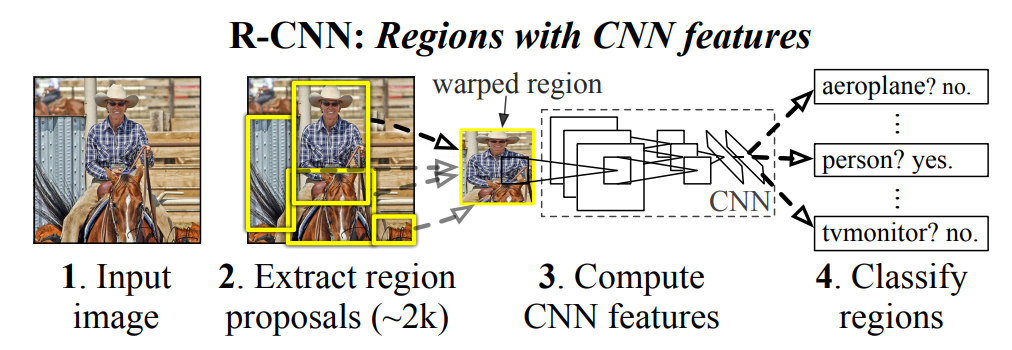
\includegraphics[width=1\textwidth]{chapter2/rcnn}
	\caption{\label{fig:2_rcnn} RCNN architecture. Image from \citet{rcnn}.}
\end{figure}

\subsection{SPPNet \cite{sppnet}}
SPPNet, shown in fig \ref{fig:2_sppnet}, takes a different approach than R-CNN. Conventional CNN-based methods are limited by the fact that the fully connected layers at the end of the network require a fixed input size. This means that the input image has to be resized to a fixed size for each region, which leads to loss of information and/or bad representation, this can be seen in \ref{fig:2_rcnn}. SPPNet solves this problem by adding a spatial pyramid pooling layer (SPP) after the last convolutional layer, a comparison with conventional CCNs can be found in fig \ref{fig:2_sppnetvscnn}. Convolutional layers can take any size input, which is then pooled to the fixed size required for the fully connected layers by the SPP layer. As the convolutional layers are only run once per image, this greatly improves the speed of the network, reaching 20-100x speedup compared to R-CNN. The SPP layer consists of parallel max-pooling layers with differing amounts of pooling regions, which are then concatenated to form a fixed-length representation, as shown in fig \ref{fig:2_sppnet}.

\begin{figure}[H]
	\centering
	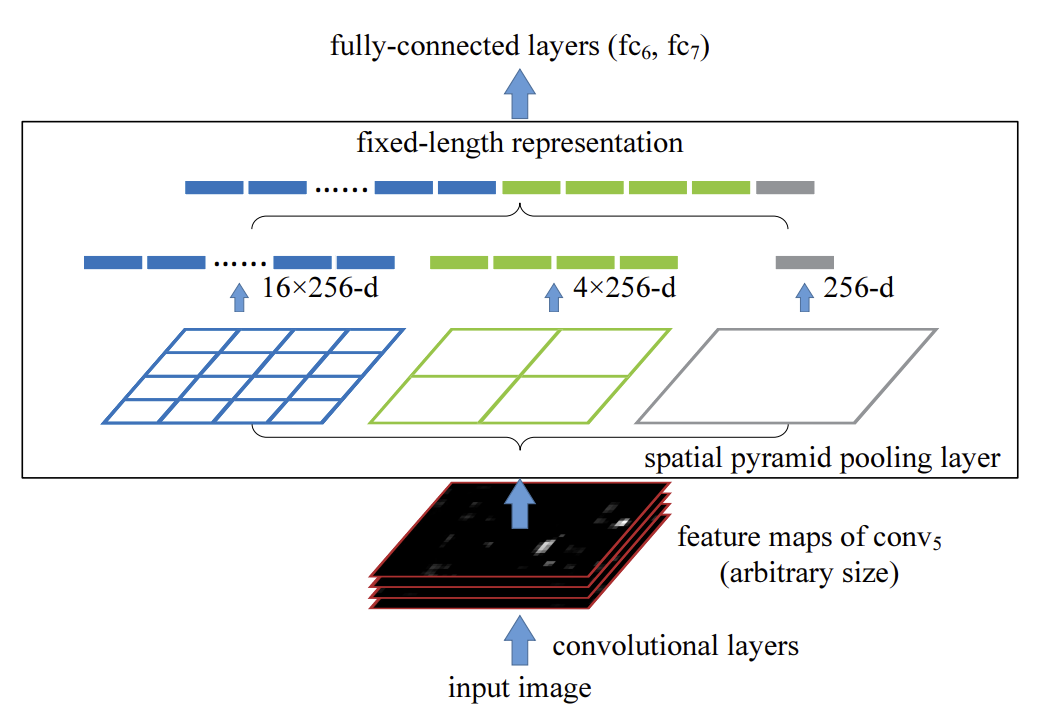
\includegraphics[width=1\textwidth]{chapter2/SPP.png}
	\caption{\label{fig:2_sppnet} SPPNet architecture. Image from \citet{sppnet}.}
\end{figure}

\begin{figure}[H]
	\centering
	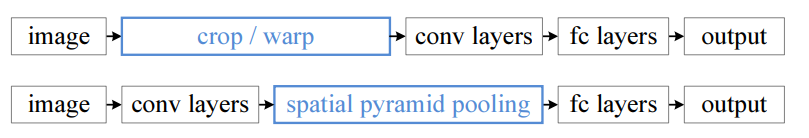
\includegraphics[width=1\textwidth]{chapter2/SPPvsCNN.png}
	\caption{\label{fig:2_sppnetvscnn} Conventional CNN vs SPPNet. Image from \citet{sppnet}.}
\end{figure}

\subsection{Fast R-CNN \cite{fastrcnn}}
Fast R-CNN, shown in fig \ref{fig:2_fastrcnn}, combines the region proposals of R-CNN with the method of SPPNet. It runs the CNN on the whole image and then applies max pooling for each region proposal, they call this region of interest pooling (RoI pooling). The RoI layer is a special case of the SPP layer, the case where the number of pooling regions is 1. As the time-consuming CNN is only run once per image, the training and inference time is greatly improved, while the RoI pooling layer increases the accuracy of the network.

\begin{figure}[H]
	\centering
	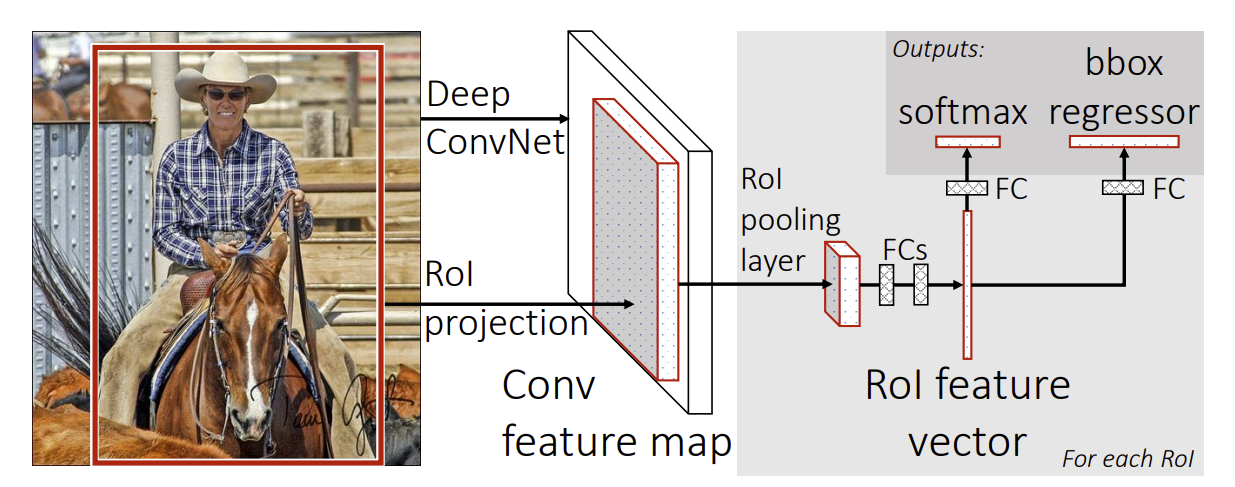
\includegraphics[width=1\textwidth]{chapter2/fastrcnn.png}
	\caption{\label{fig:2_fastrcnn} Fast R-CNN architecture. Image from \citet{fastrcnn}.}
\end{figure}

\subsection{Faster R-CNN \cite{fasterrcnn}}
Faster R-CNN, shown in fig \ref{fig:2_fasterrcnn}, improves on Fast R-CNN by replacing the region proposal method with a region proposal network (RPN). The RPN is a fully convolutional network that takes the feature map from the CNN and outputs a set of rectangular object proposals, each with an objectness score. The RPN is trained end-to-end with the rest of the network, which allows the network to learn the region proposal method that works best for the task at hand. This greatly improves the speed of the network, as the RPN is much faster than the region proposal method used in Fast R-CNN.

\begin{figure}[H]
	\centering
	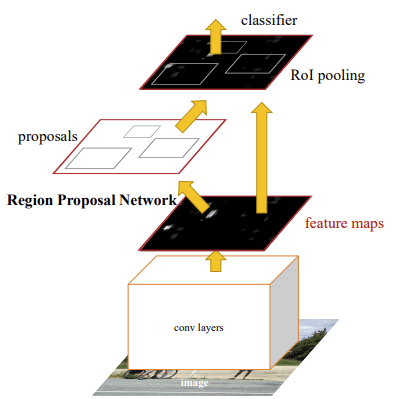
\includegraphics[width=0.6\textwidth]{chapter2/fasterrcnn.png}
	\caption{\label{fig:2_fasterrcnn} Faster R-CNN architecture. Image from \citet{fasterrcnn}.}
\end{figure}

\subsection{Vision Transformers \cite{vit}}
In recent years, the availability of more data has led to the development of architectures that were not previously possible. One example is the transformer architecture \cite{transformers}, originally designed for natural language processing (NLP) tasks, but now also used in computer vision by \citet{vit} who call their approach Vision Transformers (ViT). ViT applies the standard transformers architecture to images with minimal changes and therefore shares most characteristics with transformers. Transformers performs best when trained on large amounts of data. ViT is pre-trained on either the ImageNet-21k dataset or the JFT-300M dataset and then fine-tuned on various benchmarks, where it exceeds the CNN-based state-of-the-art. The ViT architecture is illustrated in Figure \ref{fig:2_vit}. The model starts by dividing the image into a fixed number of patches, which are linearly projected into a 1D vector. To account for the position of each patch, a position embedding is added to the input.

\begin{figure}[H]
	\centering
	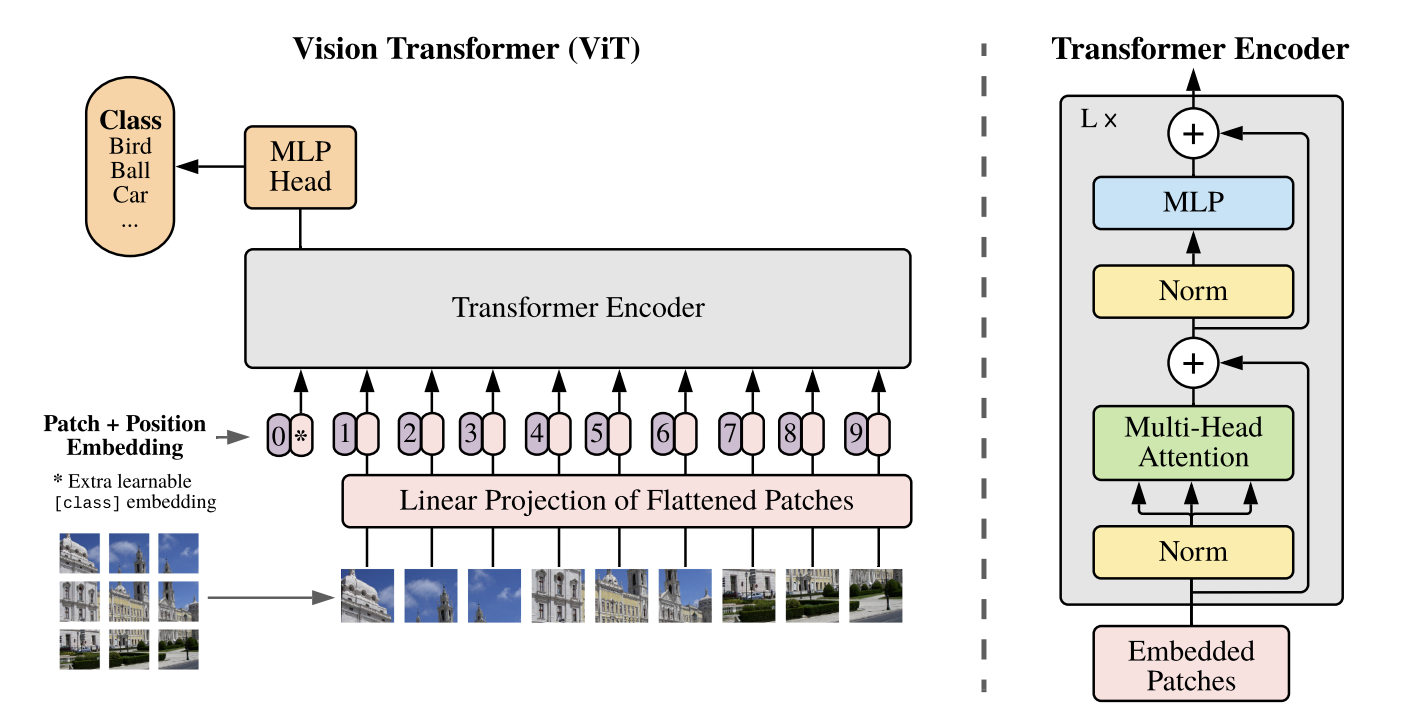
\includegraphics[width=0.8\textwidth]{chapter2/vit.png}
	\caption{\label{fig:2_vit} ViT architecture. Image from \citet{vit}.}
\end{figure}

\subsection{Transformers \cite{transformers}}
As ViT uses transformers, it is important to understand how they work. The transformers architecture was introduced by \citet{transformers} in Attention is all you need. It uses a traditional encoder-decoder structure but foregoes all convolutional layers for attention layers and fully connected layers. The encoder consists of two sub-layers for each layer, a multi-head self-attention layer and a fully connected feed-forward network. Each sub-layer has a residual connection and a layer normalization layer. The decoder is similar to the encoder but has an additional multi-head attention layer that takes the output of the encoder as input. 

The attention layer is the most important part of the transformer architecture. It is a function that takes a set of queries, keys, and values and outputs a weighted sum of the values. The weights are calculated by taking the dot product of the query and key vectors and then applying a softmax function. The output of the attention layer is then the weighted sum of the values. The multi-head attention layer is a set of attention layers that are run in parallel, each with its own set of queries, keys, and values. The output of each attention layer is concatenated and then linearly projected to the expected dimension. The attention layer is illustrated in Figure \ref{fig:2_attention}.

\begin{figure}[H]
	\centering
	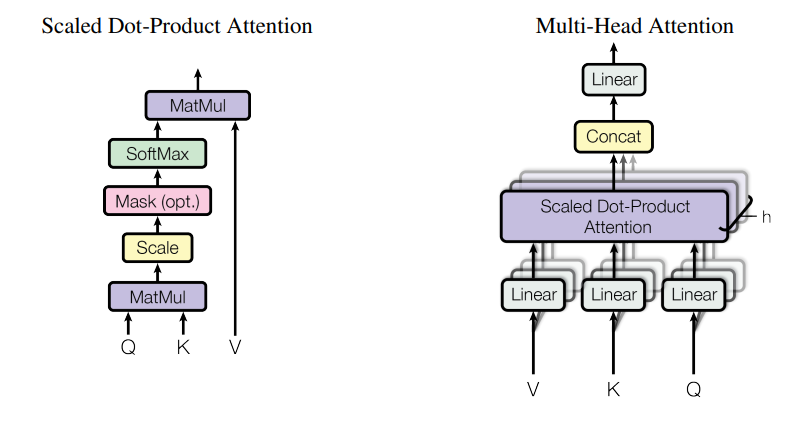
\includegraphics[width=0.8\textwidth]{chapter2/attention.png}
	\caption{\label{fig:2_attention} Attention layer. Image from \citet{transformers}.}
\end{figure}


\section{Few-shot object detection}
%https://arxiv.org/abs/2112.11699
%https://ieeexplore-ieee-org.kuleuven.e-bronnen.be/stamp/stamp.jsp?tp=&arnumber=1597116
%add a reference to the first paper that did it
Few-shot object detection is a technique that has been gaining popularity in the last few years, but interest in training a neural network to classify without a big annotated dataset appeared as early as 2008 with zero-shot learning in \citet{aaai08-132}. It allows us to train a model with few annotated images, which is useful in scenarios where it isn't possible to get a large annotated dataset. Few-shot attempts to mirror the way humans learn. During our life we come across many new objects and we are able to recognize them even though we only saw them a few times. We do this by drawing on our knowledge of other objects and using that to recognize the new object\cite{biederman1987recognition}. 

Different approaches to few-shot learning vary on a few characteristics
\begin{itemize}
	\item The type of architecture used
	\item The amount and type of data used
\end{itemize}

In this section, we will go over the different options for each of these characteristics.

\subsection{Method}

Two different methodologies can be applied to few-shot learning, transfer learning and meta-learning. Each of these has its advantages and disadvantages. %add metric learning and data augmentation

\subsubsection*{Transfer learning}

Transfer learning is a technique that has been used for a long time in machine learning. It allows us to use a model that has been trained on a large dataset as a base and, with a few changes to mitigate the small size of the novel dataset in few-shot learning, finetune (the last layers) on a novel dataset. The advantages of this method are that it is relatively easy to implement and it is fast. One of the problems with this method is that, because of the small size of the novel dataset, the Region proposal network (RPN), which provides class-agnostic bounding boxes, can not be properly trained and can sometimes completely miss the novel object classes. Mitigations for this problem do, however, exist. \cite{DBLP:journals/corr/abs-2011-10142, VU2022104398, DBLP:journals/corr/abs-2105-09491, DBLP:journals/corr/abs-2103-05950,rs14143255}.

\subsubsection*{Meta-learning}

Meta-learning learns on a higher order of abstraction. Instead of learning how to detect objects it learns how to learn to detect objects. It does this with the help of a large dataset, by learning how to best extract and differentiate the features of its classes. Due to the dataset being large, this can then be applied to a novel dataset. It is best if the novel dataset is similar to the large dataset, as it will be able to generalize better. Practically meta-learning is most commonly done by introducing a support branch\cite{few-shot-comprehensive-survey}, displayed in figure \ref{fig:2_dualbranchmeta}. An advantage of this method is that it is better at the detection of alike novel classes due to the meta loss, a loss function on the support branch. %needs citation
The disadvantages are its complexity and that it is slower to train than transfer learning due to the aforementioned support branch. As the support branch is computed once after training, it is not significantly slower during inference.
%needs sauces

\begin{figure}[H]
	\centering
	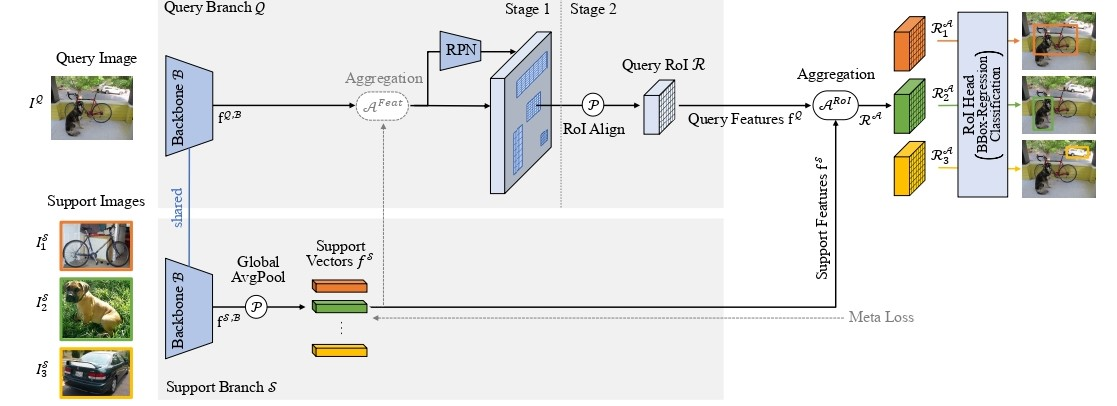
\includegraphics[width=1\textwidth]{chapter2/dualbranchmeta}
	\caption{\label{fig:2_dualbranchmeta} Dual branch meta learning. Image from \citet{few-shot-comprehensive-survey}.}
\end{figure}

\subsection{Data}

The amount and type of data used in few-shot learning is also an important factor. A common way to describe a few shot task is "N-Way, K-Shot". Where N is the number of classes and K is the number of examples per class. The more examples we have per class, the easier it is to learn. The larger the number of classes the harder. Models are often benchmarked with increasing K to see how they perform with values of K often set at (2,) 5, 10 and 30. When the amount of images decreases even further we enter a whole new category of few-shot learning, one-shot learning and zero-shot learning. Finally, the requirements for the type of annotations on the data can vary depending on the training method used. Supervised requires a fully annotated dataset, semi-supervised a partially annotated dataset and unsupervised doesn't need labels at all.

\subsubsection*{One-shot learning}

While one-shot learning is not a new concept, applying it to object detection is hard. Early applications used a siamese backbone, as is often seen in other one-shot applications, but this was not very successful \citep{One-shot-siamese}. However, recently OWL-ViT \citep{owlvit} improved one-shot object detection by a large margin, reaching 41.8 mAP for one-shot object detection on the COCO dataset. OWL-Vit will be discussed in more detail in section \ref{sec:2_owlvit}.


\section{Metrics}
In machine learning, it is important to test the model after training, to evaluate its performance. To test the model's accuracy a part of the initial dataset is split off into a test set and never used when training. As we have the ground truth for the test set we can compare it with the network output to find if the detections are correct. 

To find if the model output matches the expected output we use the Intersection over Union (IoU) metric. This compares the area of the input and output bounding boxes for each detection by dividing the area of intersection by the area of union. If the IoU, calculated as shown in \ref{eq:IoU}, is above a threshold (th) it is considered a detection.

\begin{figure}[h]
	\centering
	\documentclass{standalone}

\usepackage{tikz,pgf}

\begin{document}


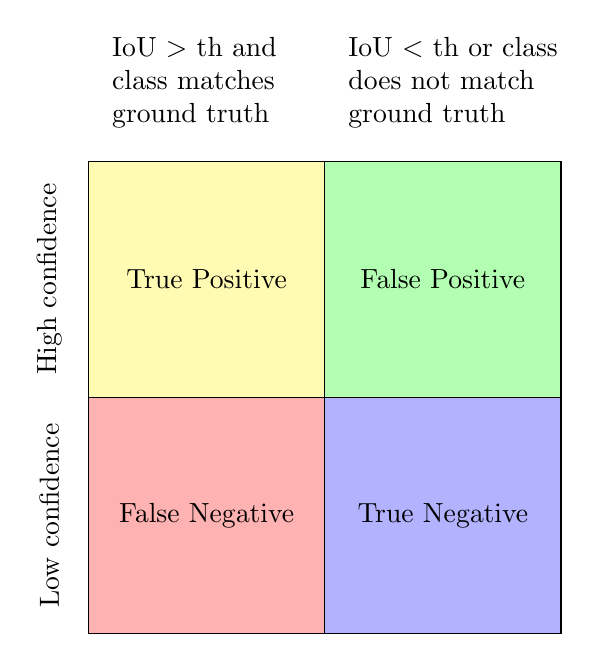
\begin{tikzpicture}
    \draw[draw=black,fill=yellow!30] (0,0) rectangle (3,3);
    \draw[draw=black,fill=green!30] (3,0) rectangle (6,3);
    \draw[draw=black,fill=red!30] (0,-3) rectangle (3,0);
    \draw[draw=black,fill=blue!30] (3,-3) rectangle (6,0);
    
    \node at (1.5,1.5) {True Positive};
    \node at (4.5,1.5) {False Positive};
    \node at (1.5,-1.5) {False Negative};
    \node at (4.5,-1.5) {True Negative};

    \node[text width=2.8cm] at (1.7,4) {IoU \begin{math}>\end{math} th and class matches ground truth};
    \node[text width=2.8cm] at (4.7,4) {IoU \begin{math}<\end{math} th or class does not match ground truth};
    \node[rotate=90] at (-0.5,1.5) {High confidence};
    \node[rotate=90] at (-0.5,-1.5) {Low confidence};
\end{tikzpicture}


\end{document}
	\caption{\label{fig:2_IoU_det} IoU and class match to find the type of detection.}
\end{figure}

\begin{equation}
	\text{IoU} = \frac{\text{area of intersection}}{\text{area of union}}
	\label{eq:IoU}
\end{equation}

Each detection can be put into one of four categories, based on if and how well it matches the ground truth, listed below.

\begin{itemize}
	\item True positive: The model correctly detects an object and the IoU is above the threshold.
	\item False positive: The model detects an object but the IoU is below the threshold or the model mislabels the object.
	\item False negative: The model does not detect an object but it should have.
	\item True negative: The model does not detect an object and it should not have, this is not used in the metrics as it is not very useful.
\end{itemize}

Using this a few key metrics can be calculated. The main metrics we will use are precision, recall and their derivatives. Precision (\ref{eq:precision}) is the ratio of true positives to the total number of positives. Recall (\ref{eq:recall}) is the ratio of true positives to the total number of detectable positives.



\begin{equation}
	Precision = \frac{TruePositives}{True Positives + False Positives}
	\label{eq:precision}
\end{equation}

\begin{equation}
	Recall = \frac{True Positives}{True Positives + False Negatives}
	\label{eq:recall}
\end{equation}

The model assigns each detection a confidence score, the dividing threshold between high and low confidence can be chosen freely. A high confidence threshold will result in a low recall but high precision. A low confidence threshold will result in a high recall but low precision. Plotting the precision and recall against the threshold results in a precision-recall curve.

Averaging the precision across all recall levels results in the average precision (AP) metric. Averaging the AP over all classes results in the mean average precision (mAP) metric. The mAP is the most common metric used to evaluate object detection models.

\section{State of the art} 
In this section, we will go over the state of the art in few-shot object detection with a focus on the previously discussed methods and types of data.

%Oneshot learning: https://arxiv.org/pdf/2205.06230v2.pdf
\subsection*{Simple Open-Vocabulary Object Detection
with Vision Transformers. (\citet{owlvit})} \label{sec:2_owlvit}

\citet{owlvit} introduce a new method, Vision Transformer for Open-World Localization, or OWL-ViT. They modify ViT to make it work for object detection instead of classification. They modify ViT after pre-training by removing the token pooling layer, which downsamples the output embeddings to optimize computation, as that doesn't work for open-vocabulary detection. It is replaced with a set of lightweight classification and box heads at each output token. The classification head does a linear projection, while the box head is a simple MLP with one hidden layer with a gelu activation function. The whole model (both text and image encoders) is then finetuned on standard object detection datasets. It is then ready to be used for one-shot object detection as it can take text, but also image-derived embeddings to find matching objects in the query image.

\begin{figure}[h]
	\centering
	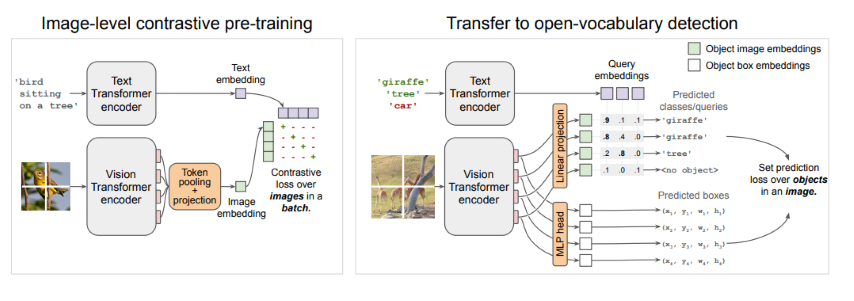
\includegraphics[width=1\textwidth]{chapter2/owlvit.png}
	\caption{\label{fig:2_owl-vitr} Original ViT to OWL-ViT. Image from \citet{owlvit}.}
\end{figure}

%K-shot(10), DETR, transfer learning, unsupervised: https://arxiv.org/pdf/2106.04550v4.pdf



%K-shot(30), ViT, transfer learning from self-supervised, fully-supervised: https://arxiv.org/pdf/2205.09613v2.pdf
\subsection*{Integrally Migrating Pre-trained Transformer Encoder-decoders
for Visual Object Detection. (\citet{imTED})}

\citet{imTED} extend the ViT architecture by making full use of the transformer encoder-decoder instead of merely using the encoder as its backbone, as many other methods do. Whereas other methods use the encoder as their backbone and initialize the FPN, RPN and detector head from scratch, imTED instead uses the decoder as its detector head. As such the only parts that need to be trained are the FPN, RPN and output layers of the FPN and decoder. The final architecture is like faster RCNN, but with the encoder as the backbone and the decoder as the detector head. The number of parameters that are randomly initialized is reduced by 81.3\%.


\begin{figure}[h]
	\centering
	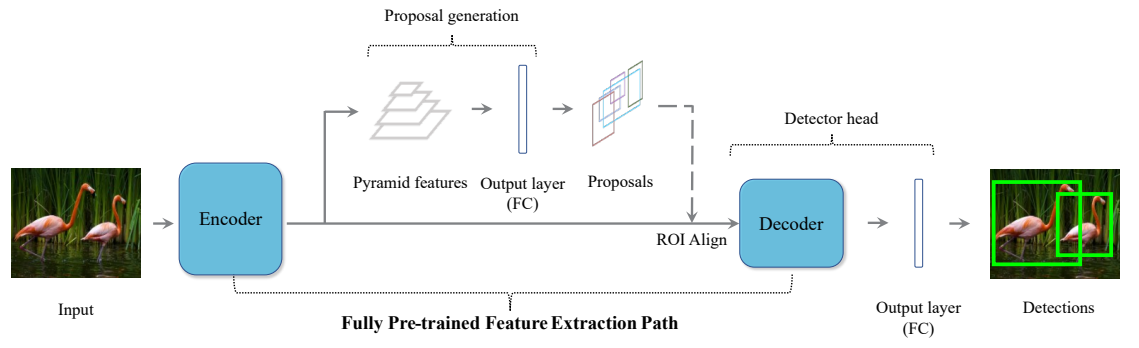
\includegraphics[width=1\textwidth]{chapter2/imTED_full}
	\caption{\label{fig:2_imTED_full} imTED architecture. Image from \citet{imTED}.}
\end{figure}

%K-shot, Faster R-CNN, meta-learning: https://arxiv.org/pdf/2208.07039v3.pdf
\subsection*{Hierarchical Attention Network for Few-Shot
Object Detection via Meta-Contrastive Learning. (\citet{hANMCL})}

\citet{hANMCL} expand upon Faster R-CNN \citep{fasterrcnn} by introducing a  hierarchical attention module (HAM) and a meta-contrastive learning module (Meta-CLM). The HAM combines the robustness of global attention with the local context information of a convolutional network by first applying local attention and then applying global attention. The stages can be found in fig \ref{fig:2_hANMCL_HAM}. The Meta-CLM combines contrastive learning with meta-learning. It works on the same principles as contrastive learning, only instead of positive and negative images it uses positive and negative image pairs. Due to being metric-based, it can be used without any finetuning on novel classes.

\begin{figure}[H]
	\centering
	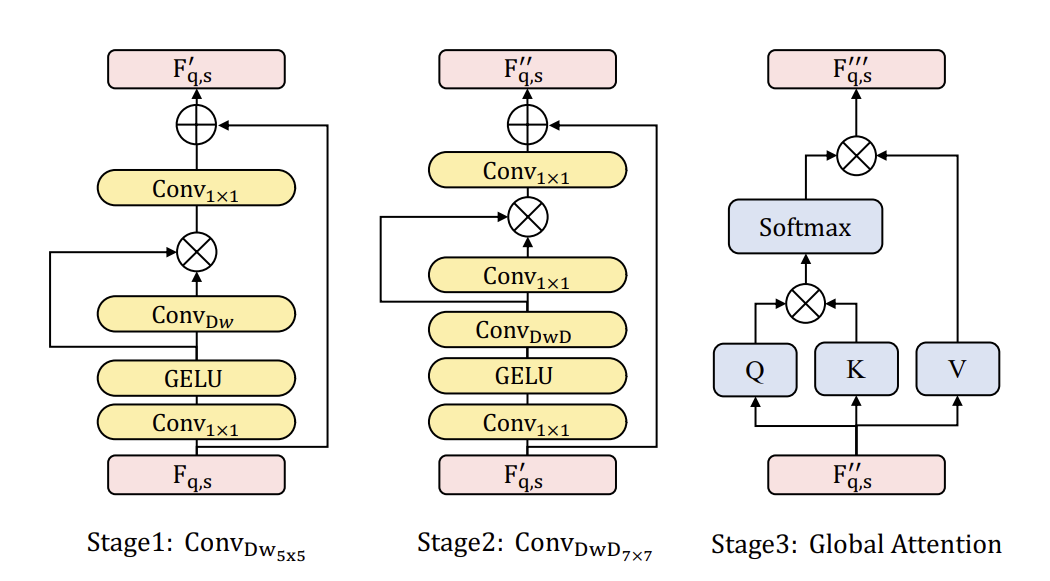
\includegraphics[width=0.7\textwidth]{chapter2/hANMCL_HAM.png}
	\caption{\label{fig:2_hANMCL_HAM} Detailed view of the HAM. Image from \citet{hANMCL}.}
\end{figure}

\begin{figure}[H]
	\centering
	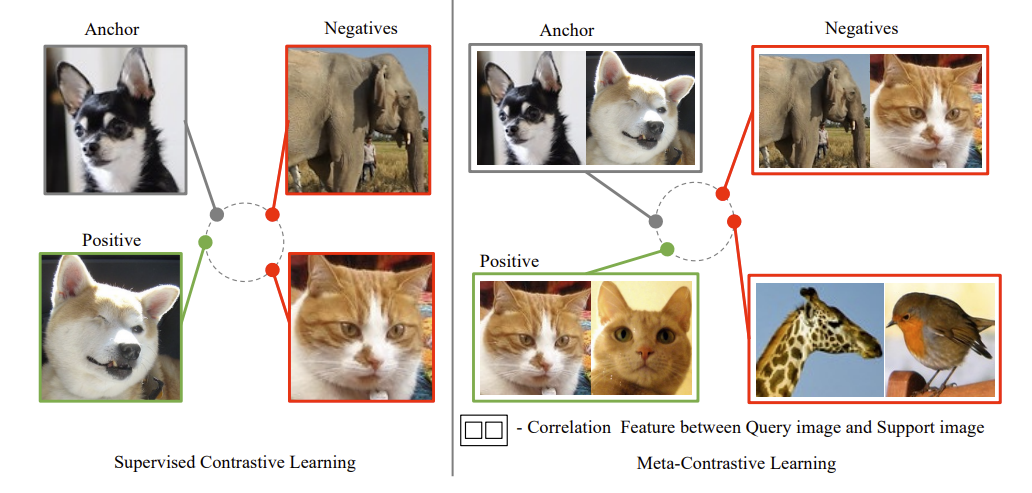
\includegraphics[width=0.8\textwidth]{chapter2/hANMCL.png}
	\caption{\label{fig:2_hANMCL} Meta-contrastive learning. Image from \citet{hANMCL}.}
\end{figure}

\section{Conclusion}

\begin{table}[H]
	\begin{tabular}{lll}\cline{2-3}
	\multicolumn{1}{l|}{}                         & \multicolumn{1}{l|}{Scores on COCO} & \multicolumn{1}{l|}{Special characteristic}\\ \hline
	\multicolumn{1}{|l|}{\multirow{3}{*}{OWL-ViT}} & \multicolumn{1}{l|}{49.1* [1 shot]}          & \multicolumn{1}{l|}{\multirow{3}{*}{1-Shot-N-Way without retraining}}\\ \cline{2-2}
	\multicolumn{1}{|l|}{}                         & \multicolumn{1}{l|}{41.8* [10 shot]}          & \multicolumn{1}{l|}{}\\ \cline{2-2}
	\multicolumn{1}{|l|}{}                         & \multicolumn{1}{l|}{/}              & \multicolumn{1}{l|}{}\\ \hline
	\multicolumn{1}{|l|}{\multirow{3}{*}{imTED}}   & \multicolumn{1}{l|}{/}              & \multicolumn{1}{l|}{\multirow{3}{*}{Reduced training time/diffuculty}}\\ \cline{2-2}
	\multicolumn{1}{|l|}{}                         & \multicolumn{1}{l|}{22.5** [10 shot]}           & \multicolumn{1}{l|}{}\\ \cline{2-2}
	\multicolumn{1}{|l|}{}                         & \multicolumn{1}{l|}{30.2** [30 shot]}           & \multicolumn{1}{l|}{}\\ \hline
	\multicolumn{1}{|l|}{\multirow{3}{*}{hANMCL}}  & \multicolumn{1}{l|}{13.4** [1 shot]}           & \multicolumn{1}{l|}{\multirow{3}{*}{\begin{tabular}[c]{@{}l@{}}1-Shot-N-Way without retraining\\ Faster R-CNN based, so less performant hardware required\\ Contrastive-learning suited to divide metric space of our alike shells\end{tabular}}} \\ \cline{2-2}
	\multicolumn{1}{|l|}{}                         & \multicolumn{1}{l|}{22.4** [10 shot]}           & \multicolumn{1}{l|}{}\\ \cline{2-2}
	\multicolumn{1}{|l|}{}                         & \multicolumn{1}{l|}{25.0** [30 shot]}           & \multicolumn{1}{l|}{}\\ \hline
	\multicolumn{3}{l}{*Results on AP50}\\
	\multicolumn{3}{l}{**Results on AP COCO}
	\end{tabular}
\end{table}
In this chapter we have studied object counting, narrowing it down to few-shot object detection to then count the detections. We went into more detail regarding the different ways to implement few-shot learning to detect objects. Studying the SOTA methods for few-shot object detection, we found that a wide variety of models, each with different advantages and disadvantages exist. OWL-ViT and hANMCL are capable of few-shot object detection without finetuning/retraining, thus they are a good fit to establish a baseline. In terms of viability, hANMCL is faster R-CNN-based and uses a convolutional backbone, as opposed to OWL-ViT and imTED which use ViT, an attention-based backbone. Both OWL-ViT as hANMCL can be used to initially establish a baseline as they do not require retraining. For our implementation we will start with finetuning hANMCL, if we have the time and hardware to do so we will also finetune OWL-ViT and imTED to compare the results.